\documentclass[11pt]{article}
\usepackage[letterpaper,margin=1in]{geometry}
\usepackage[T1]{fontenc}
\usepackage{lmodern,microtype}
\usepackage{amsmath,amssymb,booktabs,array,longtable}
\PassOptionsToPackage{svgnames}{xcolor}
\usepackage{graphicx,xcolor,tikz}
\usepackage{caption}
\usepackage[numbers,sort&compress]{natbib}
\usepackage[colorlinks=true,allcolors=blue!45!black,breaklinks=true]{hyperref}
\hypersetup{pdftitle={Law as a Verifiable Domain: Using Real-World Judicial Outcomes to Evaluate AI Legal Reasoning},pdfauthor={John J. Hughes, III},pdfsubject={Legal forecasting, probabilistic evaluation, and outcome feedback},pdfkeywords={legal AI, forecasting, benchmark, Brier score, reinforcement learning}}
\urlstyle{same}
\captionsetup{font=small,labelfont=bf}
% Drafting markers. A line starting with % TODO is visible only in the source.
% Colored macros mark provisional prose. For a clean PDF, redefine \draft,
% \checkcite, and \checknum to return their argument unchanged.
\newcommand{\draft}[1]{\textcolor{red}{#1}}
\newcommand{\checkcite}[1]{\textcolor{blue}{#1}}
\newcommand{\checknum}[1]{\textcolor{orange}{#1}}
% BEGIN GENERATED LAB REVIEW NUMBERS
% Counts from the human review of sampled Harvey LAB criteria.
\newcommand{\labTasks}{52}
\newcommand{\labCriteria}{2{,}858}
\newcommand{\labSolFlagged}{616}
\newcommand{\labOpusBlind}{650}
\newcommand{\labOpusFinal}{564}
\newcommand{\labFlagged}{835}
\newcommand{\labFlaggedPct}{29.2}
\newcommand{\labSample}{25}
\newcommand{\labSampleTasks}{19}
\newcommand{\labDefective}{16}
\newcommand{\labArguable}{3}
\newcommand{\labNotDefective}{6}
\newcommand{\labObjective}{9}
\newcommand{\labEnvItems}{14}
\newcommand{\labEnvTasks}{10}
\newcommand{\labAnyDefect}{20}
\newcommand{\labNoDefect}{4}
\newcommand{\labBothFlagged}{10}
\newcommand{\labBothDefective}{9}
\newcommand{\labSingleFlagged}{15}
\newcommand{\labSingleDefective}{7}
\newcommand{\labDefectiveLB}{383}
\newcommand{\labDefectivePoint}{534}
\newcommand{\labDefectiveShare}{13.4}
\newcommand{\labObjectiveLB}{171}
\newcommand{\labObjectivePoint}{301}
\newcommand{\labObjectiveShare}{5.9}
\newcommand{\labEnvLB}{319}
\newcommand{\labEnvShare}{11.1}
\newcommand{\labEnvPoint}{468}
\newcommand{\labAnyLB}{524}
\newcommand{\labAnyPoint}{668}
% END GENERATED LAB REVIEW NUMBERS
\setlength{\emergencystretch}{2em}
% Flush paragraphs. A gap marks a new paragraph; no line is indented.
\usepackage[skip=0.6em]{parskip}
\title{Law as a Verifiable Domain: Using Real-World\\Judicial Outcomes to Evaluate AI Legal Reasoning}
\author{John J. Hughes, III\\Independent researcher\\\url{https://www.johnjhughesiii.com/research/}}
\date{Working draft --- October 8, 2026}
\begin{document}
\maketitle
\begin{abstract}
Reinforcement learning (RL) techniques, in domains that can offer objectively verifiable rewards, have led to incredible and noteworthy recent gains in the capabilities of frontier AI models. But not all domains are equally verifiable. Many high-level legal judgment tasks are difficult to verify, and model capability gains on those tasks have not been nearly as noteworthy as model gains in domains that are susceptible to automated verification like math and coding.

This paper argues that the heavy reliance of existing legal benchmarks on human-written rubrics and artificially constructed environments fails to take advantage of key properties of the common law judicial tradition, which gives precedential effect and the force of law to reasoned judicial decisions issued by judges in specific cases or controversies. For AI researchers, those judicial dispositions supply an external signal that allows for evaluation of some high-level legal judgment tasks against an objectively verifiable real-world ground truth. In the legal system, the opinions of legal experts or data providers as to what the law is have no authoritative or precedential value. The pronouncements of a tribunal, by contrast, carry the force of law (and often precedential effect).

LegalForecastBench illustrates one mechanism by which the signal from judicial decisions can be used to objectively evaluate the legal reasoning capabilities of frontier models. Models receive the same briefs that a federal judge received when ruling on a motion to dismiss, and are asked to estimate the probability that the judge dismissed each claim challenged by a defendant.

The beta includes 91 cases and 387 scored claim--defendant units. Of the 17 frontier models tested, GPT-6 Sol has the lowest micro-Brier loss (0.118) and the highest accuracy (84.5\%). Noticeably, calibration had a significant impact on the performance of models. Claude Fable 5.1 had no errors in its 81 high-confidence (at least 90\%) forecasts, while for Gemini 3.1 Pro Preview, 57 out of 320 high-confidence predictions it made were inaccurate. In a few instances, newer model versions scored worse than their predecessors; for GPT-6.1 Sol, this was largely due to more overconfident predictions.
\end{abstract}

\section{Introduction}

Reinforcement learning (RL) techniques have led to significant recent gains in frontier model capabilities, but the most noteworthy gains have been in domains like mathematics and coding that are susceptible to automated verification. Reinforcement learning with verifiable rewards (RLVR) has allowed frontier models to gain capabilities by receiving reward signals from automated correctness checks (like mathematical answer matching, executable tests, or formal proof checking) \citep{deepseek,rlve}. Earlier self-play systems demonstrated the powerful capabilities that automated outcome feedback could provide to models playing games with explicit rules and automatable scoring mechanisms \citep{alphazero}.

Frontier models have also made noteworthy gains on legal tasks that are objectively verifiable; for example, tests that ask models bar exam-style questions about established legal propositions are approaching saturation. Neel Guha's legal benchmark dashboard reports 98.3\% accuracy (115/117) for Gemini 3 Flash on a publicly released subset of Multistate Bar Examination questions, with several other frontier models exceeding 90\% \citep{legalEval}. This increase in legal capabilities has forced researchers to develop new tasks that challenge today's frontier models. The literature illustrates at least two approaches being used recently: preference evaluation (comparing which of two outputs practicing attorneys prefer) and rubric-based reinforcement learning (grading model outputs against specified criteria to produce a reward) \citep{judgmentbench}. While these approaches are important and useful, building reliable rubric-based benchmarks for high-end legal work is extremely difficult. For example, JudgmentBench found that rubric-based scoring was less effective than attorneys' pairwise comparisons at recovering the intended quality ordering in different pieces of draft work product. OpenAI has flagged at least one benchmark that was initially useful, but later found to have specification errors once models outgrew the benchmark \citep{swecritique}. I have conducted a separate audit of the litigation tasks in Harvey's Legal Agent Benchmark and discovered errors and instances where tasks did not capture the full complexity and judgment that goes into preparing legal work product \citep{labauditpaper}. Harvey is revising those tasks, and the audit will be released alongside some revisions. These issues underscore the extraordinary difficulty of obtaining reliable, high-quality training data that can improve frontier models' legal abilities at current capability levels.

This paper aims to demonstrate that judicial dispositions in litigation matters provide a valuable external signal that can make high-level legal judgment tasks verifiable against an objective ground truth. This approach rests on a simple reality of the legal system: ``It is emphatically the province and duty of the Judicial Department to say what the law is.'' \emph{Marbury v. Madison}, 5 U.S. 137, 177 (1803). Every litigated judgment has the force of law as between the parties, and definitively resolves any disputes between the parties on the interpretation of the law or its application to a specific fact pattern.

LegalForecastBench illustrates one specific use of this signal, using judges' rulings on motions to dismiss to evaluate the predictive abilities of frontier models. The benchmark focuses on district court level motions because lower courts are heavily constrained by precedent and largely decide garden-variety disputes in which the ability to correctly analyze and apply the law to the alleged facts will be the primary way to predict the outcome. Prediction at this level is likely to serve as a reasonable proxy for legal analytical ability (whereas the U.S. Supreme Court is not nearly as constrained by precedent, since it is free to overrule any of its own prior precedential decisions, and prediction at that level would focus to a much greater extent on modeling the preferences or likely vote of individual justices). Obviously, not every judicial disposition is accurate, and there are some politically salient cases even in the lower courts where different judges might have different leanings, so the prediction task is not a pure test of legal reasoning ability.

But even so, frontier models' prediction ability is valuable and important, because prediction is a high-level legal judgment task often performed by the most senior and highly compensated lawyer on the case team because of its enormous consequences for the client's legal strategy. In many kinds of cases (such as securities fraud class actions), whether the motion to dismiss is granted or denied can have an enormous impact on the practical economic value of a case; the vast majority of cases in which pre-trial dismissal motions are denied end in settlement, whereas a case that is dismissed at the outset usually results in no recovery to the plaintiff \citep[p.~16]{securitiesFilings2024}. Prior research shows that even parties who have no intention of litigating negotiate legal resolutions ``in the shadow of the law'' \citep{shadow}. When deciding whether to settle a dispute or litigate, each side's expected value from litigation (net of the costs and risks involved) can function as a kind of reservation value; if the settlement offer is worth less than the expected value from litigation, then a party will rationally reject settlement and litigate instead. \citep{priestklein,settlement}. This can make settlement difficult or impossible if both sides are overly optimistic about their chances of success in litigation; models that help lawyers and their clients better calibrate their expectations could help unlock the enormous surplus that litigants achieve when they settle consensually (avoiding the costs, risks, and distraction brought on by protracted, adversarial litigation), by helping both sides to see their case more realistically, which should make them more willing to offer and accept the fair value of the case.

\section{Related work}


\subsection{Legal outcome prediction}
Using AI models to predict litigation outcomes has a long lineage, although the incredible recent growth in frontier model capabilities has created opportunities for more powerful approaches than those available to prior researchers. One early experiment involved the 2002 Term of the U.S. Supreme Court; Ruger and colleagues predicted the outcome of cases that Term using hand-coded metadata and statistical techniques \citep{ruger}. Later researchers used more sophisticated machine-learning and natural language processing techniques. Aletras and colleagues in 2016 used a text-based approach to predict the outcomes of European Court of Human Rights decisions \citep{aletras}. Katz, Bommarito, and Blackman in 2017 used a random-forest classifier over structured Supreme Court data to predict Justice votes and case outcomes. \citep{katz}. CAIL2018 used a dataset of more than 2.6 million Chinese criminal cases to predict charges and sentences, with text-classification models providing initial baselines. \citep{cail}. As the transformer architecture became dominant, models like BERT and T5 were increasingly used. CLC-UKET, released in 2024, compared fine-tuned BERT and T5 models to zero- and few-shot GPT-3.5 and GPT-4 to predict U.K. Employment Tribunal cases. \citep{clcuket}.

\subsection{Legal AI benchmarks and evaluation}
The growth in frontier model capabilities has similarly coincided with increasingly ambitious benchmarks. LegalBench, released in 2023, is a major collaborative benchmark to which 40 authors contributed 162 tasks intended to assess legal domain expertise. The benchmark deliberately tests relatively clean legal propositions that can be reduced to a binary answer. \citep{legalbench}.

Most recent benchmarks have sought to test higher-level judgment tasks, which usually lack an objective ground truth. JudgmentBench, released in May 2026, and Harvey's LAB targeted open-ended professional legal work, like drafting, analysis, and advice, for which there are potentially multiple defensible outputs and no independently verifiable ground truth \citep{harveyLAB,judgmentbench}. These benchmarks take different approaches to reward specification. JudgmentBench compared rubric-based scoring to comparative judgment (pairwise preference judgments collected from practicing attorneys), and found that comparative judgments recover the intended quality ordering substantially better than rubrics. LAB relies on a rubric-based approach, to allow rapid and scalable scoring of new model releases.

\subsection{Verifiable rewards, forecasting, and outcome feedback}
Frontier models are trained on several different forms of feedback, as described in prior work, including Reinforcement Learning with Verifiable Rewards (RLVR). Recent work has used real-world (nonlegal) events to supply an objective training signal for RLVR. For example, Autocast, released in 2022, gathered forecasting questions from tournaments and a date-indexed news corpus, then had language models make predictions based on the information a human would have had at the time. \citep{autocast}. Halawi and colleagues in 2024 used a retrieval-augmented forecasting system that could search for information, and generate and aggregate multiple forecasts \citep{halawi}. ForecastBench, introduced in 2024, used this approach to create a dynamic benchmark that continually collects questions about unresolved future events and scores models once the event outcome is known \citep{forecastbench}.

Outcome-Based Reinforcement Learning to Predict the Future showed in 2025 that resolved binary forecasting questions could serve as reinforcement-learning rewards, training a 14-billion-parameter model on more than 100,000 events using adaptations of GRPO and ReMax \citep{outcomerl}. OpenForecaster similarly explored training language models directly on resolved forecasting questions \citep{openforecaster}. Some research in China has also used frontier models to predict criminal sentences \citep{sentencing}.

\section{LegalForecastBench: Dataset and evaluation protocol}
% BEGIN AI-PREPARED (disclosed in the AI use statement; not sent to the Pangram check)
% TODO: No rewrite. Optional: the end of 4.1 still tells the two-model agreement and the nine dropped cases, which 4.2 also tells.

\subsection{Prediction target and information set}
Let $c\in\{1,\ldots,C\}$ index cases and $u\in\mathcal U_c$ index scored units within case $c$. Each unit identifies a challenged claim or a separately resolvable pleaded subclaim that a plaintiff has asserted against a moving defendant (or a group of similarly situated moving defendants). The ``units'' (i.e., the claims that each set of defendant(s) is moving to dismiss) are identified by labeling models that were given access to the motion papers.

When the benchmark is run, a model receives the same docket and motion papers that the judge received $X_c$ and the specification of the units that are being challenged $U_{cu}$ and returns
\begin{equation}
 p_{cu}\in[0,1],\qquad p_{cu}\approx \Pr(Y_{cu}=1\mid X_c,U_{cu}),
\end{equation}
where $Y_{cu}=1$ means that the judge dismissed that specific claim-defendant unit in its entirety, in the target motion's first written disposition. That event is not necessarily a final victory in the lawsuit: a plaintiff could be given leave to amend the complaint (in which case the defendant typically will file a renewed motion to dismiss), or other claims might survive even if some are dismissed. The plaintiff also has a right to appeal final dismissal orders.


\begin{table}[ht]
\centering\small
\begin{tabular}{p{.60\linewidth}p{.29\linewidth}}
\toprule
First written disposition of the frozen unit & Primary label \\
\midrule
Entire claim dismissed, with or without leave to amend & $1$: fully dismissed \\
Only one nonseparable theory or remedy dismissed; claim remains & $0$: not fully dismissed \\
Claim dismissed against one defendant but survives against another & Separate labels for separately frozen units \\
Disposition does not reliably resolve the frozen target & Excluded from primary scoring \\
\bottomrule
\end{tabular}
\caption{Illustrative label semantics.}
\label{tab:labels}
\end{table}

\subsection{Cohort construction and labeling}
The analyzed set consists of 91 U.S. federal cases with written decisions dated June 30--August 7, 2026. The cases, as labeled, contained 409 claim-defendant units that could be forecasted. Of those, 387 are scored. The unscored units involved situations where the plaintiff voluntarily withdrew the frozen claim, the order did not cleanly grant or deny the frozen claim, or (for four units) we determined after freezing the unit that the frozen defendant was the wrong target or the motion did not address the frozen claim. Of the scored claim-defendant units, 285 were fully dismissed and 102 were not. The sample was not random; our pipeline favored cases where some of the necessary documents could be obtained for free from online databases, although we typically still had to purchase a number of documents to obtain a complete set of the substantive motion papers that were before the judge.

The case construction and labeling pipeline used models as well as human legal oversight from me. The pipeline maintained separation between \emph{unitization} and \emph{outcome coding}. To avoid the possibility that the prediction units could leak information about the judge's ultimate outcome to the models that were performing prediction, AI models first were asked to identify the challenged claim-defendant units based only on the motion and the docket (without the decision). A later stage was given access to the judge's ruling, to interpret the disposition of each frozen claim-defendant unit. I resolved disputed units (where two models did not agree on the disposition) and corrected labels as necessary. The process of creating the pipeline was iterative, and we did not track a blinded human-audit error estimate.

Models predicting outcomes were not given access to the judge's ruling. The pipeline also attempted to screen dockets and filing text to avoid outcome leakage. Models had access to the motion to dismiss papers (through document text tools) in a sandbox with no Internet access. Model API calls were made with provider-side web search disabled. Provider-specific reasoning settings are retained in the run registries. Appendix~\ref{app:protocol} lists the configuration settings. The study population is the seventeen configurations in Table~\ref{tab:main}.

The decisions used in the benchmark were decided by the federal judges and became public, only after the reported knowledge or training cutoffs for all of the models that disclose such cutoffs. Kimi and Muse do not publish training cutoffs, but based on the model release dates, it appears unlikely that those models were exposed to the decisions in training.

The acquisition and labeling pipeline is designed to create new cohorts in the future, as new judicial decisions become available. This enables fresh comparisons even after models have been trained on the specific decisions at issue here. The downside of this approach is that refreshing the benchmark with a new cohort of cases changes the case mix and difficulty, so scores from different versions cannot be interpreted as a time series of model improvement.

\subsection{Scoring and statistical inference}
For $N=\sum_c |\mathcal U_c|=387$ and $C=91$, the primary metric is the micro-Brier loss
\begin{equation}
 B_{\mathrm{micro}}=\frac{1}{N}\sum_{c=1}^C\sum_{u\in\mathcal U_c}(p_{cu}-Y_{cu})^2.
\label{eq:micro}
\end{equation}
The equal-case score changes the estimand by giving each case the same weight:
\begin{equation}
 B_{\mathrm{case}}=\frac{1}{C}\sum_{c=1}^C\frac{1}{|\mathcal U_c|}\sum_{u\in\mathcal U_c}(p_{cu}-Y_{cu})^2.
\label{eq:case}
\end{equation}
Lower is better for both. Micro-Brier treats each scored claim--defendant unit equally, so cases that involve a motion to dismiss many separate claims receive more weight than cases where only one claim and defendant was subject to a motion to dismiss. Equal-case Brier weights each prediction unit in inverse proportion to the number of units from that case.

The Brier rule is strictly proper for the binary target. If the true conditional event probability is $q$, then
\begin{equation}
 \mathbb E[(p-Y)^2\mid X,U]=(p-q)^2+q(1-q),
\label{eq:proper}
\end{equation}
which is minimized by reporting $p=q$. The second term is irreducible uncertainty for that information set. A set of observable judicial events therefore creates a verifiable score across the entire probability distribution, even though a single realized outcome standing alone does not reveal whether the probability a model assigned to that outcome was correct ex ante \citep{brier,gneiting}. Accuracy at threshold $p\geq0.5$ is reported as a secondary descriptive metric.

The observed dismissal frequency is $\widehat\pi=285/387=0.73643$. Always predicting dismissal has accuracy 73.64\%, so a constant forecast $p=\widehat\pi$ has micro-Brier $\widehat\pi(1-\widehat\pi)=0.19410$. The constant is fitted retrospectively on this cohort, so it is a descriptive reference, not a baseline derived from earlier cases. The uninformative forecast $p=0.5$ has Brier 0.25.

Log loss is a complementary diagnostic:
\begin{equation}
 L=-\frac{1}{N}\sum_{c,u}\left[Y_{cu}\log p_{cu}+(1-Y_{cu})\log(1-p_{cu})\right].
\end{equation}
For a wrong forecast assigning 0.99 to the predicted class, Brier loss is 0.9801 and log loss is approximately 4.605; at confidence 0.90 the corresponding losses are 0.81 and 2.303. Thus log loss imposes a large penalty on instances where the model assigned a very high probability to the outcome that did not occur.

Claim--defendant units from the same case share facts and legal issues; distinct claims in a single case may suffer from closely related legal defects, so the outcomes are not independent. We therefore measure within-case dependence using an observed-scale intraclass correlation coefficient (ICC) \citep{makicc}.

% BEGIN GENERATED CLUSTERING
Across the 387 scored units in 91 cases, the observed-scale outcome ICC was 0.76 (95\% CI: 0.61--0.87). Prediction losses also clustered within case because if a model failed to account, for example, for the possibility that a given motion might be denied on procedural grounds, all of the claims in a case that it expected to be dismissed could survive: GPT-6 Sol's Brier-loss ICC was 0.42 (95\% CI: 0.24--0.58). These intervals use 20,000 whole-case bootstrap resamples, and assume independence between cases.
% END GENERATED CLUSTERING
% END AI-PREPARED

\section{Results}
% BEGIN AI-PREPARED (disclosed in the AI use statement; not sent to the Pangram check)
% TODO: No rewrite. Leave this section empirical. Do not add interpretation between the subsections.

\subsection{Model performance and unconditional references}
Table~\ref{tab:main} reports the seventeen configurations on the ranked leaderboard. GPT-6 Sol achieves the best observed micro-Brier (0.11763), equal-case Brier (0.12949), and accuracy (327/387, 84.50\%). All seventeen beat the retrospectively fitted constant micro-Brier of 0.19410; GPT-6 Sol's micro-Brier is lower than that constant by about 39.4\%.

Sixteen configurations also beat majority-class accuracy (the 73.64\% accuracy of predicting dismissal for every unit). Muse Spark 1.3 does not: 279/387 correct forecasts is 72.09\%. Gemini 3.1 Pro Preview has the highest micro-Brier in the panel (0.18345) and still beats that accuracy baseline (302/387, 78.04\%). Within model families, some newer versions scored worse than older versions of the models (GPT-6.1 Sol vs.\ GPT-6 Sol, Claude Opus 5.5 vs.\ Opus 5, Claude Sonnet 5.5 vs.\ Sonnet 5 on Brier score, Grok 4.7 vs.\ 4.6, and GPT-6 Luna vs.\ GPT-5.6 Luna). None of the differences that could be tested was significant after correction for multiple comparisons; the Grok and Luna pairs could not be tested because unit-level forecasts for Grok 4.6 and GPT-5.6 Luna were not preserved.

\begin{table}[tb]
\centering\small
\setlength{\tabcolsep}{4pt}
\begin{tabular}{lrrrrr}\toprule
Configuration & Micro Brier & Case Brier & Correct & Acc. (\%) & Cost (\$)\\\midrule
GPT-6 Sol & 0.11763 & 0.12949 & 327/387 & 84.50 & 11.01 \\
Claude Fable 5.1 & 0.12877 & 0.13653 & 318/387 & 82.17 & 83.18 \\
Grok 4.6 & 0.13368 & 0.13480 & 312/387 & 80.62 & 15.72 \\
Claude Opus 5 & 0.13987 & 0.13548 & 310/387 & 80.10 & 45.89 \\
GPT-5.6 Sol & 0.14009 & 0.13319 & 313/387 & 80.88 & 24.91 \\
Kimi K3 & 0.14130 & 0.15367 & 303/387 & 78.29 & 16.87 \\
GPT-5.6 Luna & 0.14322 & 0.15084 & 313/387 & 80.88 & 1.48 \\
Claude Opus 5.5 & 0.14540 & 0.14762 & 299/387 & 77.26 & 20.59 \\
GPT-6.1 Sol & 0.14948 & 0.13885 & 304/387 & 78.55 & 10.68 \\
GPT-6 Astra & 0.15221 & 0.14275 & 305/387 & 78.81 & 59.74 \\
Gemini 3.8 Flash & 0.15331 & 0.13900 & 310/387 & 80.10 & 35.61 \\
Grok 4.7 & 0.15833 & 0.16454 & 298/387 & 77.00 & 33.00 \\
Claude Sonnet 5 & 0.15848 & 0.15964 & 293/387 & 75.71 & 24.68 \\
GPT-6 Luna & 0.16368 & 0.17379 & 296/387 & 76.49 & 0.62 \\
Claude Sonnet 5.5 & 0.17298 & 0.17183 & 295/387 & 76.23 & 6.99 \\
Muse Spark 1.3 & 0.18121 & 0.17845 & 279/387 & 72.09 & 8.78 \\
Gemini 3.1 Pro Preview & 0.18345 & 0.18080 & 302/387 & 78.04 & 59.04 \\
\midrule
Cohort-rate reference & 0.19410 & --- & 285/387 & 73.64 & ---\\
Constant $p=0.5$ & 0.25000 & 0.25000 & --- & --- & ---\\
\bottomrule\end{tabular}
\caption{Benchmark results, sorted by micro-Brier loss.}
\label{tab:main}
\end{table}

\begin{figure}[tb]\centering
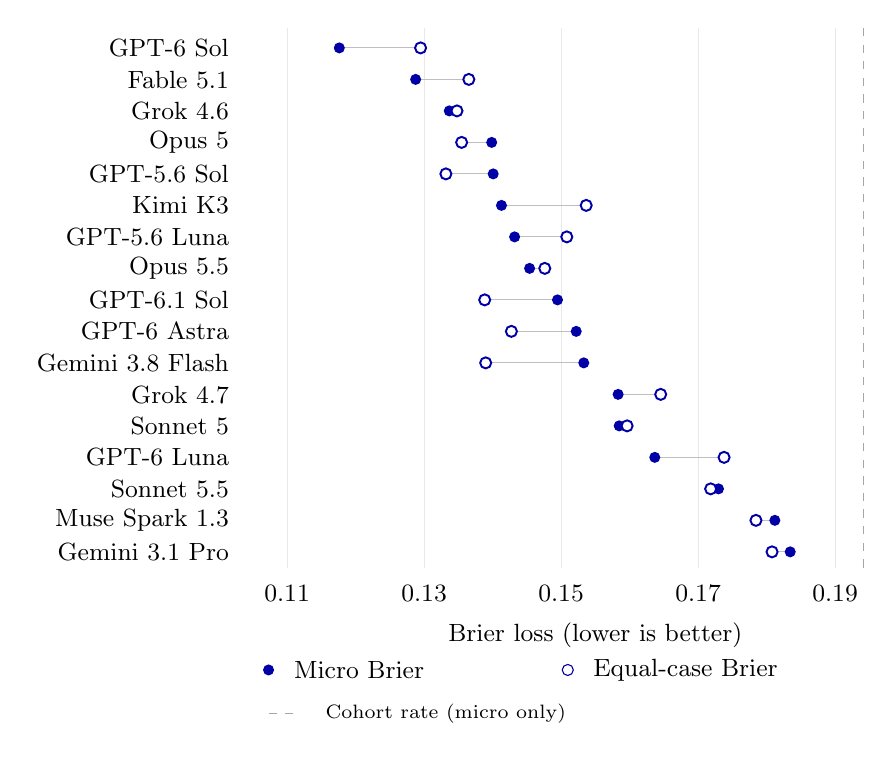
\begin{tikzpicture}[every node/.style={font=\small}]
\draw[gray!18] (0.43500,-.2)--(0.43500,6.65000);
\node[anchor=north] at (0.43500,-.3) {0.11};
\draw[gray!18] (2.17500,-.2)--(2.17500,6.65000);
\node[anchor=north] at (2.17500,-.3) {0.13};
\draw[gray!18] (3.91500,-.2)--(3.91500,6.65000);
\node[anchor=north] at (3.91500,-.3) {0.15};
\draw[gray!18] (5.65500,-.2)--(5.65500,6.65000);
\node[anchor=north] at (5.65500,-.3) {0.17};
\draw[gray!18] (7.39500,-.2)--(7.39500,6.65000);
\node[anchor=north] at (7.39500,-.3) {0.19};
\draw[dashed,gray!70] (7.75160,-.2)--(7.75160,6.65000);
\node[anchor=east] at (-.18,0.000) {Gemini 3.1 Pro};
\draw[gray!50] (6.82512,0.000)--(6.59447,0.000);
\fill[blue!65!black] (6.82512,0.000) circle (2pt);
\draw[blue!65!black,fill=white,line width=.7pt] (6.59447,0.000) circle (2pt);
\node[anchor=east] at (-.18,0.400) {Muse Spark 1.3};
\draw[gray!50] (6.62998,0.400)--(6.38993,0.400);
\fill[blue!65!black] (6.62998,0.400) circle (2pt);
\draw[blue!65!black,fill=white,line width=.7pt] (6.38993,0.400) circle (2pt);
\node[anchor=east] at (-.18,0.800) {Sonnet 5.5};
\draw[gray!50] (5.91407,0.800)--(5.81460,0.800);
\fill[blue!65!black] (5.91407,0.800) circle (2pt);
\draw[blue!65!black,fill=white,line width=.7pt] (5.81460,0.800) circle (2pt);
\node[anchor=east] at (-.18,1.200) {GPT-6 Luna};
\draw[gray!50] (5.10507,1.200)--(5.98509,1.200);
\fill[blue!65!black] (5.10507,1.200) circle (2pt);
\draw[blue!65!black,fill=white,line width=.7pt] (5.98509,1.200) circle (2pt);
\node[anchor=east] at (-.18,1.600) {Sonnet 5};
\draw[gray!50] (4.65311,1.600)--(4.75361,1.600);
\fill[blue!65!black] (4.65311,1.600) circle (2pt);
\draw[blue!65!black,fill=white,line width=.7pt] (4.75361,1.600) circle (2pt);
\node[anchor=east] at (-.18,2.000) {Grok 4.7};
\draw[gray!50] (4.63933,2.000)--(5.18010,2.000);
\fill[blue!65!black] (4.63933,2.000) circle (2pt);
\draw[blue!65!black,fill=white,line width=.7pt] (5.18010,2.000) circle (2pt);
\node[anchor=east] at (-.18,2.400) {Gemini 3.8 Flash};
\draw[gray!50] (4.20331,2.400)--(2.95760,2.400);
\fill[blue!65!black] (4.20331,2.400) circle (2pt);
\draw[blue!65!black,fill=white,line width=.7pt] (2.95760,2.400) circle (2pt);
\node[anchor=east] at (-.18,2.800) {GPT-6 Astra};
\draw[gray!50] (4.10730,2.800)--(3.28403,2.800);
\fill[blue!65!black] (4.10730,2.800) circle (2pt);
\draw[blue!65!black,fill=white,line width=.7pt] (3.28403,2.800) circle (2pt);
\node[anchor=east] at (-.18,3.200) {GPT-6.1 Sol};
\draw[gray!50] (3.86964,3.200)--(2.94516,3.200);
\fill[blue!65!black] (3.86964,3.200) circle (2pt);
\draw[blue!65!black,fill=white,line width=.7pt] (2.94516,3.200) circle (2pt);
\node[anchor=east] at (-.18,3.600) {Opus 5.5};
\draw[gray!50] (3.51502,3.600)--(3.70814,3.600);
\fill[blue!65!black] (3.51502,3.600) circle (2pt);
\draw[blue!65!black,fill=white,line width=.7pt] (3.70814,3.600) circle (2pt);
\node[anchor=east] at (-.18,4.000) {GPT-5.6 Luna};
\draw[gray!50] (3.32487,4.000)--(3.98765,4.000);
\fill[blue!65!black] (3.32487,4.000) circle (2pt);
\draw[blue!65!black,fill=white,line width=.7pt] (3.98765,4.000) circle (2pt);
\node[anchor=east] at (-.18,4.400) {Kimi K3};
\draw[gray!50] (3.15799,4.400)--(4.23419,4.400);
\fill[blue!65!black] (3.15799,4.400) circle (2pt);
\draw[blue!65!black,fill=white,line width=.7pt] (4.23419,4.400) circle (2pt);
\node[anchor=east] at (-.18,4.800) {GPT-5.6 Sol};
\draw[gray!50] (3.05295,4.800)--(2.45220,4.800);
\fill[blue!65!black] (3.05295,4.800) circle (2pt);
\draw[blue!65!black,fill=white,line width=.7pt] (2.45220,4.800) circle (2pt);
\node[anchor=east] at (-.18,5.200) {Opus 5};
\draw[gray!50] (3.03378,5.200)--(2.65210,5.200);
\fill[blue!65!black] (3.03378,5.200) circle (2pt);
\draw[blue!65!black,fill=white,line width=.7pt] (2.65210,5.200) circle (2pt);
\node[anchor=east] at (-.18,5.600) {Grok 4.6};
\draw[gray!50] (2.49521,5.600)--(2.59299,5.600);
\fill[blue!65!black] (2.49521,5.600) circle (2pt);
\draw[blue!65!black,fill=white,line width=.7pt] (2.59299,5.600) circle (2pt);
\node[anchor=east] at (-.18,6.000) {Fable 5.1};
\draw[gray!50] (2.06804,6.000)--(2.74354,6.000);
\fill[blue!65!black] (2.06804,6.000) circle (2pt);
\draw[blue!65!black,fill=white,line width=.7pt] (2.74354,6.000) circle (2pt);
\node[anchor=east] at (-.18,6.400) {GPT-6 Sol};
\draw[gray!50] (1.09863,6.400)--(2.13074,6.400);
\fill[blue!65!black] (1.09863,6.400) circle (2pt);
\draw[blue!65!black,fill=white,line width=.7pt] (2.13074,6.400) circle (2pt);
\node[anchor=north] at (4.35,-.78) {Brier loss (lower is better)};
\fill[blue!65!black] (.2,-1.5) circle(2pt);\node[anchor=west] at (.4,-1.5) {Micro Brier};
\draw[blue!65!black,fill=white] (4.0,-1.5) circle(2pt);\node[anchor=west] at (4.2,-1.5) {Equal-case Brier};
\draw[dashed,gray!70] (.2,-2.05)--(.6,-2.05);\node[anchor=west,font=\scriptsize] at (.8,-2.05) {Cohort rate (micro only)};\end{tikzpicture}
\caption{Micro- and equal-case Brier scores for the same seventeen configurations.}\label{fig:ranking}\end{figure}

\subsection{Confidence and calibration}
Define confidence $h_{cu}=\max(p_{cu},1-p_{cu})$ and the high-confidence subset $H_m=\{(c,u):h_{cu}\geq0.9\}$ for configuration $m$. Comparing the mean confidence in $H_m$ with classification accuracy in $H_m$ gives a useful conditional calibration diagnostic. Of course, this is not a full reliability curve; the subset differs by model, and its units remain clustered by case.

OpenAI models appeared more likely than others to make high-confidence forecasts. GPT-5.6 Sol, GPT-5.6 Luna, and Astra make high-confidence forecasts on 58.9\%, 47.0\%, and 53.5\% of units respectively, compared with 20.9\% for Fable 5.1. Their mean confidence in those subsets is approximately 95--97\%, while realized accuracy is approximately 89--90\%, suggesting some overconfidence, particularly for Astra, which missed 21 of 207 such predictions. Gemini 3.8 Flash also had relatively high sharpness, making 276 high-confidence forecasts (71.3\% of units) and missing 35. Gemini 3.1 Pro Preview is sharper still, making 320 high-confidence forecasts and missing 57. GPT-6 Sol provides a useful counterexample within OpenAI, missing 8 of 169 high-confidence forecasts, for 95.3\% subset accuracy. GPT-6.1 Sol is sharper and less accurate in that subset, missing 18 of 199. GPT-6 Luna misses 19 of 183. Claude Opus 5.5 misses none of 65. 

\begin{figure}[tb]\centering
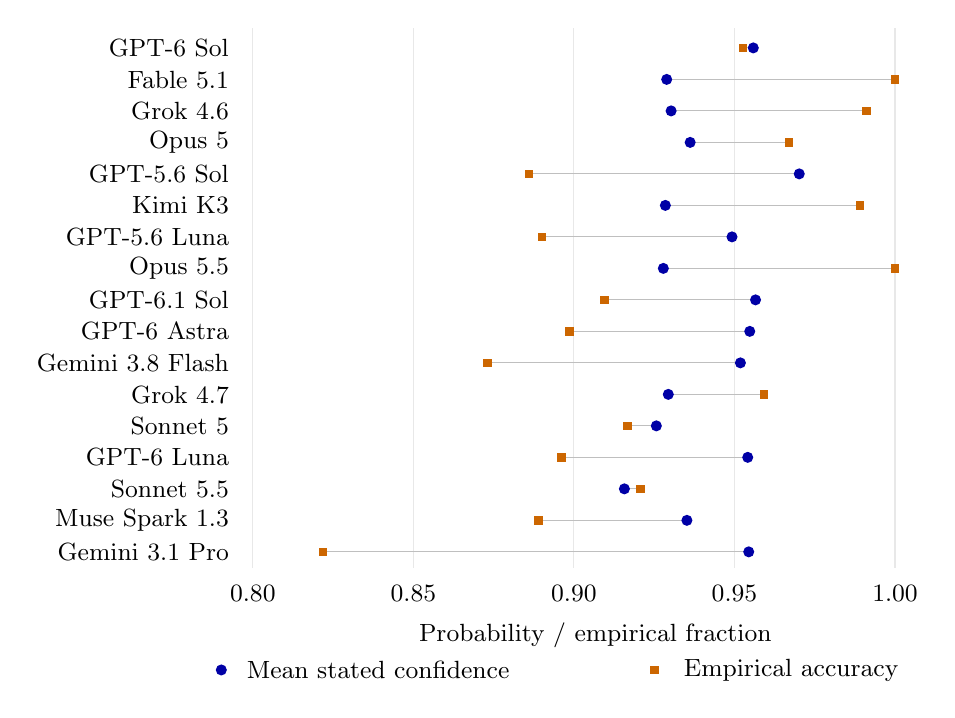
\begin{tikzpicture}[every node/.style={font=\small}]
\draw[gray!18] (0.00000,-.2)--(0.00000,6.65000);
\node[anchor=north] at (0.00000,-.3) {0.80};
\draw[gray!18] (2.03906,-.2)--(2.03906,6.65000);
\node[anchor=north] at (2.03906,-.3) {0.85};
\draw[gray!18] (4.07812,-.2)--(4.07812,6.65000);
\node[anchor=north] at (4.07812,-.3) {0.90};
\draw[gray!18] (6.11719,-.2)--(6.11719,6.65000);
\node[anchor=north] at (6.11719,-.3) {0.95};
\draw[gray!18] (8.15625,-.2)--(8.15625,6.65000);
\node[anchor=north] at (8.15625,-.3) {1.00};
\node[anchor=east] at (-.18,0.000) {Gemini 3.1 Pro};
\draw[gray!50] (6.29815,0.000)--(0.89209,0.000);
\fill[blue!65!black] (6.29815,0.000) circle (2pt);
\fill[orange!80!black] (0.83709,-0.055) rectangle (0.94709,0.055);
\node[anchor=east] at (-.18,0.400) {Muse Spark 1.3};
\draw[gray!50] (5.51302,0.400)--(3.62500,0.400);
\fill[blue!65!black] (5.51302,0.400) circle (2pt);
\fill[orange!80!black] (3.57000,0.345) rectangle (3.68000,0.455);
\node[anchor=east] at (-.18,0.800) {Sonnet 5.5};
\draw[gray!50] (4.71897,0.800)--(4.91964,0.800);
\fill[blue!65!black] (4.71897,0.800) circle (2pt);
\fill[orange!80!black] (4.86464,0.745) rectangle (4.97464,0.855);
\node[anchor=east] at (-.18,1.200) {GPT-6 Luna};
\draw[gray!50] (6.28544,1.200)--(3.92213,1.200);
\fill[blue!65!black] (6.28544,1.200) circle (2pt);
\fill[orange!80!black] (3.86713,1.145) rectangle (3.97713,1.255);
\node[anchor=east] at (-.18,1.600) {Sonnet 5};
\draw[gray!50] (5.12484,1.600)--(4.75781,1.600);
\fill[blue!65!black] (5.12484,1.600) circle (2pt);
\fill[orange!80!black] (4.70281,1.545) rectangle (4.81281,1.655);
\node[anchor=east] at (-.18,2.000) {Grok 4.7};
\draw[gray!50] (5.27659,2.000)--(6.49171,2.000);
\fill[blue!65!black] (5.27659,2.000) circle (2pt);
\fill[orange!80!black] (6.43671,1.945) rectangle (6.54671,2.055);
\node[anchor=east] at (-.18,2.400) {Gemini 3.8 Flash};
\draw[gray!50] (6.19254,2.400)--(2.98471,2.400);
\fill[blue!65!black] (6.19254,2.400) circle (2pt);
\fill[orange!80!black] (2.92971,2.345) rectangle (3.03971,2.455);
\node[anchor=east] at (-.18,2.800) {GPT-6 Astra};
\draw[gray!50] (6.31124,2.800)--(4.01902,2.800);
\fill[blue!65!black] (6.31124,2.800) circle (2pt);
\fill[orange!80!black] (3.96402,2.745) rectangle (4.07402,2.855);
\node[anchor=east] at (-.18,3.200) {GPT-6.1 Sol};
\draw[gray!50] (6.38462,3.200)--(4.46749,3.200);
\fill[blue!65!black] (6.38462,3.200) circle (2pt);
\fill[orange!80!black] (4.41249,3.145) rectangle (4.52249,3.255);
\node[anchor=east] at (-.18,3.600) {Opus 5.5};
\draw[gray!50] (5.21373,3.600)--(8.15625,3.600);
\fill[blue!65!black] (5.21373,3.600) circle (2pt);
\fill[orange!80!black] (8.10125,3.545) rectangle (8.21125,3.655);
\node[anchor=east] at (-.18,4.000) {GPT-5.6 Luna};
\draw[gray!50] (6.08582,4.000)--(3.67479,4.000);
\fill[blue!65!black] (6.08582,4.000) circle (2pt);
\fill[orange!80!black] (3.61979,3.945) rectangle (3.72979,4.055);
\node[anchor=east] at (-.18,4.400) {Kimi K3};
\draw[gray!50] (5.23950,4.400)--(7.71298,4.400);
\fill[blue!65!black] (5.23950,4.400) circle (2pt);
\fill[orange!80!black] (7.65798,4.345) rectangle (7.76798,4.455);
\node[anchor=east] at (-.18,4.800) {GPT-5.6 Sol};
\draw[gray!50] (6.93979,4.800)--(3.50576,4.800);
\fill[blue!65!black] (6.93979,4.800) circle (2pt);
\fill[orange!80!black] (3.45076,4.745) rectangle (3.56076,4.855);
\node[anchor=east] at (-.18,5.200) {Opus 5};
\draw[gray!50] (5.55434,5.200)--(6.80811,5.200);
\fill[blue!65!black] (5.55434,5.200) circle (2pt);
\fill[orange!80!black] (6.75311,5.145) rectangle (6.86311,5.255);
\node[anchor=east] at (-.18,5.600) {Grok 4.6};
\draw[gray!50] (5.31249,5.600)--(7.79213,5.600);
\fill[blue!65!black] (5.31249,5.600) circle (2pt);
\fill[orange!80!black] (7.73713,5.545) rectangle (7.84713,5.655);
\node[anchor=east] at (-.18,6.000) {Fable 5.1};
\draw[gray!50] (5.25625,6.000)--(8.15625,6.000);
\fill[blue!65!black] (5.25625,6.000) circle (2pt);
\fill[orange!80!black] (8.10125,5.945) rectangle (8.21125,6.055);
\node[anchor=east] at (-.18,6.400) {GPT-6 Sol};
\draw[gray!50] (6.35608,6.400)--(6.22578,6.400);
\fill[blue!65!black] (6.35608,6.400) circle (2pt);
\fill[orange!80!black] (6.17078,6.345) rectangle (6.28078,6.455);
\node[anchor=north] at (4.35,-.78) {Probability / empirical fraction};
\fill[blue!65!black] (-.4,-1.5) circle(2pt);\node[anchor=west] at (-.2,-1.5) {Mean stated confidence};
\fill[orange!80!black] (5.05,-1.555) rectangle(5.16,-1.445);\node[anchor=west] at (5.35,-1.5) {Empirical accuracy};\end{tikzpicture}
\caption{Conditional confidence diagnostic on predictions with $\max(p,1-p)\geq0.9$. Each row uses the subset selected by that model, rather than a common set of units. Wrong/selected counts: GPT-6 Sol: 8/169; Fable 5.1: 0/81; Grok 4.6: 1/112; Opus 5: 4/121; GPT-5.6 Sol: 26/228; Kimi K3: 1/92; GPT-5.6 Luna: 20/182; Opus 5.5: 0/65; GPT-6.1 Sol: 18/199; GPT-6 Astra: 21/207; Gemini 3.8 Flash: 35/276; Grok 4.7: 4/98; Sonnet 5: 5/60; GPT-6 Luna: 19/183; Sonnet 5.5: 5/63; Muse Spark 1.3: 15/135; Gemini 3.1 Pro: 57/320. This is not a full reliability diagram or an estimate of statistical significance.}\label{fig:confidence}\end{figure}

Other high-performing models were less sharp. For example, Fable has no errors among 81 high-confidence units, while Kimi and Grok 4.6 each miss one. Claude Sonnet 5.5 makes 63 high-confidence forecasts and misses 5. The practical finding is that confidence varies substantially and it materially affects proper scores. Astra's underperformance relative to cheaper models like Sol, for example, appears largely due to several high-confidence misses, which resulted in large Brier losses.


\subsection{Evaluating Jev, a non-autoregressive discriminative decision model}
Jev---described by its developer as a probabilistic ``System One'' model---was evaluated as a separate experiment because its context window and lack of agentic tool calling differ from the document-enabled configurations used with frontier models. \citep{jevdocs}. GPT-5.6 Luna summarized the motion documents, without commentary or analysis. Jev received the summaries, and the unit questions, in a single request per case, without document tools or multiple turns. In a second condition, Grok 4.6 prepared a separate set of shorter summaries of the same 482 documents, which Jev received under the same protocol.
\begin{table}[tb]\centering\small
\begin{tabular}{lrrr}\toprule
Condition & Micro Brier & Case Brier & Acc. (\%)\\\midrule
GPT-5.6 Luna full documents & 0.14322 & 0.15084 & 80.88 \\
GPT-5.6 Luna summary + high reasoning & 0.15489 & 0.16119 & 78.55 \\
GPT-6 Luna summary + no reasoning & 0.17152 & 0.18694 & 74.16 \\
Jev Luna summary + one-shot & 0.36754 & 0.34416 & 32.56 \\
Jev Grok summary + one-shot & 0.32725 & 0.30505 & 38.24 \\
\bottomrule\end{tabular}
\caption{Results from the Jev experiment, with Luna evaluating the same Luna summaries as a control. No control received the Grok summaries.}
\label{tab:summary}\end{table}
\begin{figure}[tb]\centering
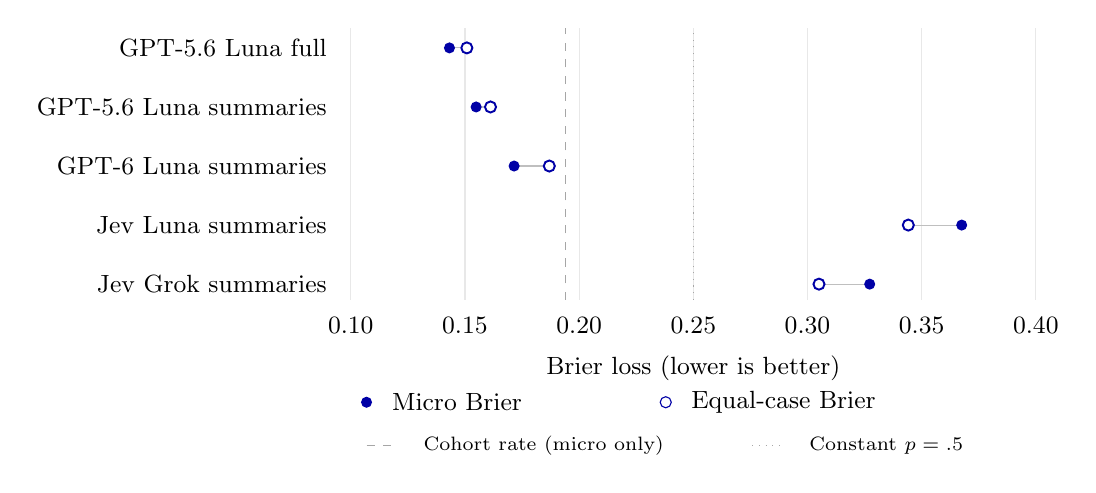
\begin{tikzpicture}[every node/.style={font=\small}]
\draw[gray!18] (0.00000,-.2)--(0.00000,3.250);
\node[anchor=north] at (0.00000,-.3) {0.10};
\draw[gray!18] (1.45000,-.2)--(1.45000,3.250);
\node[anchor=north] at (1.45000,-.3) {0.15};
\draw[gray!18] (2.90000,-.2)--(2.90000,3.250);
\node[anchor=north] at (2.90000,-.3) {0.20};
\draw[gray!18] (4.35000,-.2)--(4.35000,3.250);
\node[anchor=north] at (4.35000,-.3) {0.25};
\draw[gray!18] (5.80000,-.2)--(5.80000,3.250);
\node[anchor=north] at (5.80000,-.3) {0.30};
\draw[gray!18] (7.25000,-.2)--(7.25000,3.250);
\node[anchor=north] at (7.25000,-.3) {0.35};
\draw[gray!18] (8.70000,-.2)--(8.70000,3.250);
\node[anchor=north] at (8.70000,-.3) {0.40};
\draw[dashed,gray!70] (2.72887,-.2)--(2.72887,3.250);
\draw[dotted,gray!70] (4.35000,-.2)--(4.35000,3.250);
\node[anchor=east] at (-.18,0.000) {Jev Grok summaries};
\draw[gray!50] (6.59031,0.000)--(5.94637,0.000);
\fill[blue!65!black] (6.59031,0.000) circle (2pt);
\draw[blue!65!black,fill=white,line width=.7pt] (5.94637,0.000) circle (2pt);
\node[anchor=east] at (-.18,0.750) {Jev Luna summaries};
\draw[gray!50] (7.75870,0.750)--(7.08070,0.750);
\fill[blue!65!black] (7.75870,0.750) circle (2pt);
\draw[blue!65!black,fill=white,line width=.7pt] (7.08070,0.750) circle (2pt);
\node[anchor=east] at (-.18,1.500) {GPT-6 Luna summaries};
\draw[gray!50] (2.07411,1.500)--(2.52134,1.500);
\fill[blue!65!black] (2.07411,1.500) circle (2pt);
\draw[blue!65!black,fill=white,line width=.7pt] (2.52134,1.500) circle (2pt);
\node[anchor=east] at (-.18,2.250) {GPT-5.6 Luna summaries};
\draw[gray!50] (1.59194,2.250)--(1.77464,2.250);
\fill[blue!65!black] (1.59194,2.250) circle (2pt);
\draw[blue!65!black,fill=white,line width=.7pt] (1.77464,2.250) circle (2pt);
\node[anchor=east] at (-.18,3.000) {GPT-5.6 Luna full};
\draw[gray!50] (1.25329,3.000)--(1.47422,3.000);
\fill[blue!65!black] (1.25329,3.000) circle (2pt);
\draw[blue!65!black,fill=white,line width=.7pt] (1.47422,3.000) circle (2pt);
\node[anchor=north] at (4.35,-.78) {Brier loss (lower is better)};
\fill[blue!65!black] (.2,-1.5) circle(2pt);\node[anchor=west] at (.4,-1.5) {Micro Brier};
\draw[blue!65!black,fill=white] (4.0,-1.5) circle(2pt);\node[anchor=west] at (4.2,-1.5) {Equal-case Brier};
\draw[dashed,gray!70] (.2,-2.05)--(.6,-2.05);\node[anchor=west,font=\scriptsize] at (.8,-2.05) {Cohort rate (micro only)};\draw[dotted,gray!70] (5.1,-2.05)--(5.5,-2.05);\node[anchor=west,font=\scriptsize] at (5.7,-2.05) {Constant $p=.5$};\end{tikzpicture}
\caption{Probability quality with a shared summary cache. Both Luna conditions exploit predictive signal in the summaries, while Jev scores worse than the constant $p=0.5$ forecast with either set of summaries. The full-document reference changes both information access and interaction. Connecting segments indicate weighting sensitivity, not uncertainty intervals.}\label{fig:summary}\end{figure}

Jev was not well-calibrated for this task. Jev's micro-Brier of 0.36754 is worse than the 0.25 loss of always reporting $p=0.5$. Its mean predicted dismissal probability was approximately 0.305, while the observed frequency in this data set was 0.736. This resulted in severe underprediction in the aggregate. Its 32.6\% threshold accuracy is also below majority-class prediction.

We tested Luna using the same summaries that Jev received in order to determine whether Jev's underperformance was attributable to receiving only summaries of the litigation documents, rather than the full documents used in our primary evaluation. Luna performed much better than Jev, even when it only had access to the same summary Jev received. GPT-5.6 Luna with the identical summaries achieves micro-Brier 0.15489 and accuracy 78.6\%, demonstrating that the summaries contained useful predictive signal that Jev was unable to exploit (although Luna performed better in the primary evaluation, where it had full document access, which could mean that the summaries lost some relevant signal or that the interactive environment allows for better performance).

We also tested whether a different summary pipeline would change Jev's result. With the Grok summaries, Jev improved to micro-Brier 0.32725, equal-case Brier 0.30505, and 38.2\% accuracy; the improvement over Jev with Luna summaries is significant on all three metrics (paired case-cluster bootstrap, Bonferroni-corrected across the six pairs of the four summary conditions and three metrics). Jev nevertheless remained significantly worse than both Luna summary controls and worse than the constant $p=0.5$ forecast; its mean predicted dismissal probability rose only to about 0.356. Because Grok wrote different summaries and no Luna control received them, this compares pipelines; it does not isolate summary quality or model ability.
% END AI-PREPARED

\section{Conclusion}

LegalForecastBench is one illustration of how real-world litigation data can be used as a reward signal with an objective ground truth to evaluate frontier models on high-level legal analytical tasks. I will soon be publishing an analysis of the existing leading legal benchmark, Harvey's Legal Agent Benchmark. Next steps in my research include testing whether these signals are also useful as training; some early results suggest that merely training on the Brier score loss function may not be a sufficiently dense reward signal to improve model performance, but we are testing techniques that might exploit more of the judge's written reasoning to create a richer task, where the model is asked to make several predictions, to create potentially denser rewards.

Even so, this experiment suggests that there are still lots of sources of training signal that have not been exploited and that could meaningfully improve the evaluation of, and performance of, frontier models. 

\section*{Reproducibility, access, and AI use disclosure}
Code is maintained in the \href{https://github.com/johnhughes3/LegalForecastBench}{LegalForecastBench repository}; documents used in the benchmark evaluation, including the documents I purchased in order to complete the evaluation, have been made available to the public through \href{https://www.courtlistener.com/}{CourtListener}. I am also happy to provide copies of the litigation documents as they were shown to models to interested researchers.

As I am a practicing attorney and do not have any formal training in artificial intelligence or machine learning, the use of AI models was essential to allow me to make a research contribution in this space that otherwise would have been beyond my capabilities. My personal contribution included the benchmark design, labeling cases for the benchmark in instances where frontier models reached differing conclusions about the correct label, and orchestrating AI coding agents that helped write and execute the code that ran the benchmark evaluation, starting on May 18, 2026, and continuing through at least October 6, 2026. I wrote most of this paper personally, but discussed the results at several points with AI agents and considered AI-generated analysis as an input into my thinking as I drafted. The major exception to this was sections 3 and 4 and other places where numerical results or mathematical notations are included; I relied on AI agents to write code that performs the necessary mathematical calculations and to prepare the LaTeX source summarizing those mathematical results. I used several different models from Anthropic, OpenAI, SpaceXAI, and Google to check the work. I also met with experienced researchers in the space to validate the experimental design and results, and obtain feedback on the draft. I am grateful to several AI researchers in industry positions for helpful discussions, and to Prof. Dr. Daniel Katz, professor of law at Illinois Tech's Chicago-Kent College of Law, for reviewing an early draft and discussing relevant findings from his prior Supreme Court prediction research. This version of the paper is intended as a working draft, and feedback from researchers, lawyers, and others on how to improve this benchmark or make our findings more useful is welcome.


\clearpage

\begin{thebibliography}{99}

\bibitem{deepseek} Daya Guo, Dejian Yang, Haowei Zhang et al. DeepSeek-R1 incentivizes reasoning in LLMs through reinforcement learning. \emph{Nature 645, 633--638 (2025); arXiv:2501.12948v2}, 2025. \url{https://www.nature.com/articles/s41586-025-09422-z}.

\bibitem{rlve} Zhiyuan Zeng, Hamish Ivison, Yiping Wang et al. RLVE: Scaling Up Reinforcement Learning for Language Models with Adaptive Verifiable Environments. \emph{ICML 2026, Proceedings of Machine Learning Research 306:153406--153428}, 2026. \url{https://proceedings.mlr.press/v306/zeng26j.html}.

\bibitem{alphazero} David Silver, Thomas Hubert, Julian Schrittwieser et al. Mastering Chess and Shogi by Self-Play with a General Reinforcement Learning Algorithm. \emph{arXiv:1712.01815 (2017), preprint; precursor to the distinct 2018 Science article}, 2017. \url{https://arxiv.org/abs/1712.01815}.

\bibitem{judgmentbench} Russell Yang, Ruishi Chen, Pierce Kelaita et al. JudgmentBench: Comparing Rubric and Preference Evaluation for Quality Assessment. \emph{arXiv:2605.25240v3, preprint}, 2026. \url{https://arxiv.org/abs/2605.25240}.

\bibitem{swecritique} OpenAI. Why SWE-bench Verified no longer measures frontier coding capabilities. \emph{Primary online source}, 2026. \url{https://openai.com/index/why-we-no-longer-evaluate-swe-bench-verified/}.

\bibitem{legalbench} Neel Guha, Julian Nyarko, Daniel E. Ho et al. LegalBench: A Collaboratively Built Benchmark for Measuring Legal Reasoning in Large Language Models. \emph{NeurIPS 2023, Datasets and Benchmarks}, 2023. \url{https://arxiv.org/abs/2308.11462}.

\bibitem{legalEval} Neel Guha. Legal LLM Leaderboard: Tracking LLM Performance on Academic Legal Benchmarks. \emph{Public evaluation dashboard; results generated April 8, 2026, accessed October 6, 2026}. BarExam: 117 publicly released Multistate Bar Examination questions. \url{https://neelguha.github.io/legal-benchmark-dashboard/}.

\bibitem{brier} Glenn W. Brier. Verification of Forecasts Expressed in Terms of Probability. \emph{Monthly Weather Review 78(1) (1950), 1--3}, 1950. \url{https://journals.ametsoc.org/view/journals/mwre/78/1/1520-0493_1950_078_0001_vofeit_2_0_co_2.xml}.

\bibitem{gneiting} Tilmann Gneiting, Adrian E. Raftery. Strictly Proper Scoring Rules, Prediction, and Estimation. \emph{Journal of the American Statistical Association 102 (2007), 359--378}, 2007. \url{https://doi.org/10.1198/016214506000001437}.

\bibitem{securitiesFilings2024} Cornerstone Research and Stanford Law School Securities Class Action Clearinghouse. Securities Class Action Filings---2024 Year in Review. \emph{Research report}, 2025. p.~16, status of core federal securities class action filings as of the end of 2024. \url{https://securities.stanford.edu/research-reports/1996-2024/Securities-Class-Action-Filings-2024-Year-in-Review.pdf}.

\bibitem{shadow} Robert H. Mnookin and Lewis Kornhauser. Bargaining in the Shadow of the Law: The Case of Divorce. \emph{Yale Law Journal}, 88(5):950--997, 1979. \url{https://doi.org/10.2307/795824}.

\bibitem{outcomerl} Benjamin Turtel, Danny Franklin, Kris Skotheim et al. Outcome-based Reinforcement Learning to Predict the Future. \emph{Transactions on Machine Learning Research (November 2025); arXiv:2505.17989v4}, 2025. \url{https://arxiv.org/abs/2505.17989}.

\bibitem{openforecaster} Nikhil Chandak, Shashwat Goel, Ameya Prabhu et al. Scaling Open-Ended Reasoning To Predict the Future. \emph{arXiv:2512.25070v2 (January 2026); preprint}, 2026. \url{https://arxiv.org/abs/2512.25070}.

\bibitem{sentencing} Junjie Chen, Haitao Li, Qilei Zhang et al. Multi-Source Retrieval and Reasoning for Legal Sentencing Prediction. \emph{arXiv:2602.04690v3; arXiv record comments 'EMNLP 2026 main' (publisher proceedings record not independently checked)}, 2026. \url{https://arxiv.org/abs/2602.04690}.

\bibitem{ruger} Theodore W. Ruger, Pauline T. Kim, Andrew D. Martin, Kevin M. Quinn. The Supreme Court Forecasting Project: Legal and Political Science Approaches to Predicting Supreme Court Decision-Making. \emph{Columbia Law Review 104 (2004), 1150--1210}, 2004. \href{https://andrewdmartin.wustl.edu/app/uploads/2019/01/The-Supreme-Court-Forecasting-Project-Legal-and-Political-Science-Approaches-to-Predicting-Supreme-Court-Decision-Making-2bvpcdb.pdf}{Author-hosted article PDF}.

\bibitem{katz} Daniel Martin Katz, Michael J. Bommarito II, Josh Blackman. A General Approach for Predicting the Behavior of the Supreme Court of the United States. \emph{PLOS ONE 12(4): e0174698 (2017)}, 2017. \url{https://journals.plos.org/plosone/article?id=10.1371%2Fjournal.pone.0174698}.

\bibitem{aletras} Nikolaos Aletras, Dimitrios Tsarapatsanis, Daniel Preotiuc-Pietro, Vasileios Lampos. Predicting Judicial Decisions of the European Court of Human Rights: A Natural Language Processing Perspective. \emph{PeerJ Computer Science 2:e93 (2016)}, 2016. \url{https://peerj.com/articles/cs-93/}.

\bibitem{cail} Chaojun Xiao, Haoxi Zhong, Zhipeng Guo et al. CAIL2018: A Large-Scale Legal Dataset for Judgment Prediction. \emph{arXiv:1807.02478 (2018); CAIL challenge dataset paper}, 2018. \url{https://arxiv.org/abs/1807.02478}.

\bibitem{clcuket} Huiyuan Xie, Felix Steffek, Joana Ribeiro de Faria et al. The CLC-UKET Dataset: Benchmarking Case Outcome Prediction for the UK Employment Tribunal. \emph{Proceedings of the Natural Legal Language Processing Workshop (ACL), 2024, pp. 81--96}, 2024. \url{https://aclanthology.org/2024.nllp-1.7/}.

\bibitem{harveyLAB} Niko Grupen, Gabe Pereyra, Julio Pereyra. Introducing Harvey's Legal Agent Benchmark. \emph{Primary online source}, 2026. \url{https://www.harvey.ai/blog/introducing-harveys-legal-agent-benchmark}.

\bibitem{autocast} Andy Zou, Tristan Xiao, Ryan Jia et al. Forecasting Future World Events with Neural Networks. \emph{NeurIPS 2022, Datasets and Benchmarks}, 2022. \url{https://arxiv.org/abs/2206.15474}.

\bibitem{halawi} Danny Halawi, Fred Zhang, Chen Yueh-Han, Jacob Steinhardt. Approaching Human-Level Forecasting with Language Models. \emph{ICML 2024, Proceedings of Machine Learning Research 235}, 2024. \url{https://arxiv.org/abs/2402.18563}.

\bibitem{forecastbench} Ezra Karger, Houtan Bastani, Chen Yueh-Han et al. ForecastBench: A Dynamic Benchmark of AI Forecasting Capabilities. \emph{ICLR2025}, 2025. \url{https://arxiv.org/abs/2409.19839}.

\bibitem{jevdocs} TypeSafe AI. Models: Jev and the System One Interface. \emph{Product documentation, accessed September 29, 2026}, 2026. \url{https://docs.typesafe.ai/models}.

\bibitem{priestklein} George L. Priest, Benjamin Klein. The Selection of Disputes for Litigation. \emph{Journal of Legal Studies 13 (1984), 1--55}, 1984. \url{https://www.journals.uchicago.edu/doi/10.1086/467732}.

\bibitem{settlement} Lucian A. Bebchuk. Litigation and Settlement Under Imperfect Information. \emph{RAND Journal of Economics 15(3) (1984), 404--415}, 1984. \url{https://hls.harvard.edu/bibliography/litigation-and-settlement-under-imperfect-information/}.

\bibitem{makicc} Tak K. Mak. Analysing Intraclass Correlation for Dichotomous Variables. \emph{Journal of the Royal Statistical Society, Series C (Applied Statistics)}, 37(3):344--352, 1988. \url{https://doi.org/10.2307/2347309}.

\bibitem{labauditpaper} John J. Hughes, III. The Challenge of Deriving Signal from Synthetic Legal Environments: Evidence from Harvey's Legal Agent Benchmark. \emph{Working paper, forthcoming}, 2026.

\end{thebibliography}

\clearpage

\appendix
\section{Model configuration and temporal evidence}
\label{app:cutoffs}\label{app:protocol}
``K'' denotes a reported knowledge cutoff, ``T'' a reported training cutoff, and ``?'' no established cutoff. Month-only dates are compared as the first day of the reported month. The reported cutoffs for fifteen configurations precede June 30, 2026. Kimi and Muse did not publish a training-data cutoff, but based on the release dates, it appears unlikely that these models would have trained on any data in our benchmark set.
\begin{table}[ht]\centering\small\setlength{\tabcolsep}{4pt}
\begin{tabular}{llll}\toprule
Configuration & Reasoning & Reported cutoff & Relation to window\\\midrule
GPT-6 Sol & High & 2026-04-20 (K) & Precedes window \\
Claude Fable 5.1 & Adaptive/default & 2026-06 (T) & Precedes window \\
Grok 4.6 & High & 2026-02-01 (K) & Precedes window \\
Claude Opus 5 & Adaptive/default & 2026-05 (T) & Precedes window \\
GPT-5.6 Sol & High & 2026-02-16 (K) & Precedes window \\
Kimi K3 & High & Unknown (?) & Unknown \\
GPT-5.6 Luna & High & 2026-02-16 (K) & Precedes window \\
Claude Opus 5.5 & High & 2026-06 (T) & Precedes window \\
GPT-6.1 Sol & High & 2026-04-30 (K) & Precedes window \\
GPT-6 Astra & High & 2026-04-30 (K) & Precedes window \\
Gemini 3.8 Flash & High & 2026-03 (K) & Precedes window \\
Grok 4.7 & High & 2026-05 (K) & Precedes window \\
Claude Sonnet 5 & Adaptive/default & 2026-01 (T) & Precedes window \\
GPT-6 Luna & High & 2026-05-18 (K) & Precedes window \\
Claude Sonnet 5.5 & High & 2026-06 (T) & Precedes window \\
Muse Spark 1.3 & High & Unknown (?) & Unknown \\
Gemini 3.1 Pro Preview & High & 2025-01 (K) & Precedes window \\
\bottomrule\end{tabular}\caption{Model Configuration and Training Cutoff Dates}\label{tab:cutoffs}\end{table}

Claude Fable 5.1, Claude Opus 5, and Claude Sonnet 5 used adaptive thinking at provider defaults. Claude Opus 5.5 and Claude Sonnet 5.5 used high effort. The other configurations use the high reasoning or thinking setting.

\section{Result provenance}
We standardized costs in the table based on the recorded token usage and standard API rates. To calculate the costs for Fable (which was inadvertently run without cache enabled), we calculated cached execution based on the turn-by-turn token usage data, rather than the original uncached usage.

The results were produced with \href{https://github.com/johnhughes3/LegalForecastBench/tree/58371a0e13494e591710e2eae3da8e428eebc359}{LegalForecastBench \texttt{58371a0e}}.

\subsection{Main Results Costs}
% BEGIN AI-PREPARED (disclosed in the AI use statement; not sent to the Pangram check)
The normalized costs range from \$0.62 for GPT-6 Luna to \$83.18 for Fable. These are not actual invoice charges. For example, Fable was initially run without caching, resulting in an actual cost of \$189.70. The normalized price was reconstructed after the fact using turn-by-turn token counts, with the reconstruction validated against real billing data from other Anthropic model runs. In several other cases, provider discounts that we received were normalized to standard API rates. On these standardized estimates, GPT-6 Luna, GPT-5.6 Luna, and GPT-6 Sol form the observed micro-Brier cost--score frontier.
% END AI-PREPARED

\subsection{Jev Evaluation Costs}
% BEGIN AI-PREPARED (disclosed in the AI use statement; not sent to the Pangram check)
Summary preparation cost an estimated \$10.32 for the Luna summaries and \$29.99 for the Grok summaries, both reconstructed from recorded usage. An earlier Grok preparation under the standard summary prompt cost a further \$2.00, and \$4.11 in uncertain Grok preparation charges is held separately and excluded from these totals. Successful inference estimates are approximately \$0.044 for Jev with Luna summaries, \$0.020 for Jev with Grok summaries (provider-reported), \$1.62 for GPT-5.6 Luna (with high reasoning), and \$0.103 for GPT-6 Luna (which was run without reasoning as a control).
% END AI-PREPARED

\end{document}
